\section{Our Approach}
	\label{section:app}
	Our work aims to develop an entity alignment model for any two arbitrary (heterogeneous) \KGs. . Without loss of generality, we
introduce our approach using two \KGs: $G_1 = (E_1,V_1,R_1,A_1,T_1)$ and $G_2 = (E_2,V_2,R_2,A_2,T_2)$ for entity alignment, where
$E,V,R,A,T$ represent entities, values, relations, attributes and triples respectively. 	We put $G_1$ and $G_2$ together in one large
graph $G$. We utilize pre-aligned entity pairs to train our models and then discover new equivalent entities. Figure~\ref{all} demonstrates
the overall architecture of our model. 	
	
	\begin{figure}[t!]
		\centering
			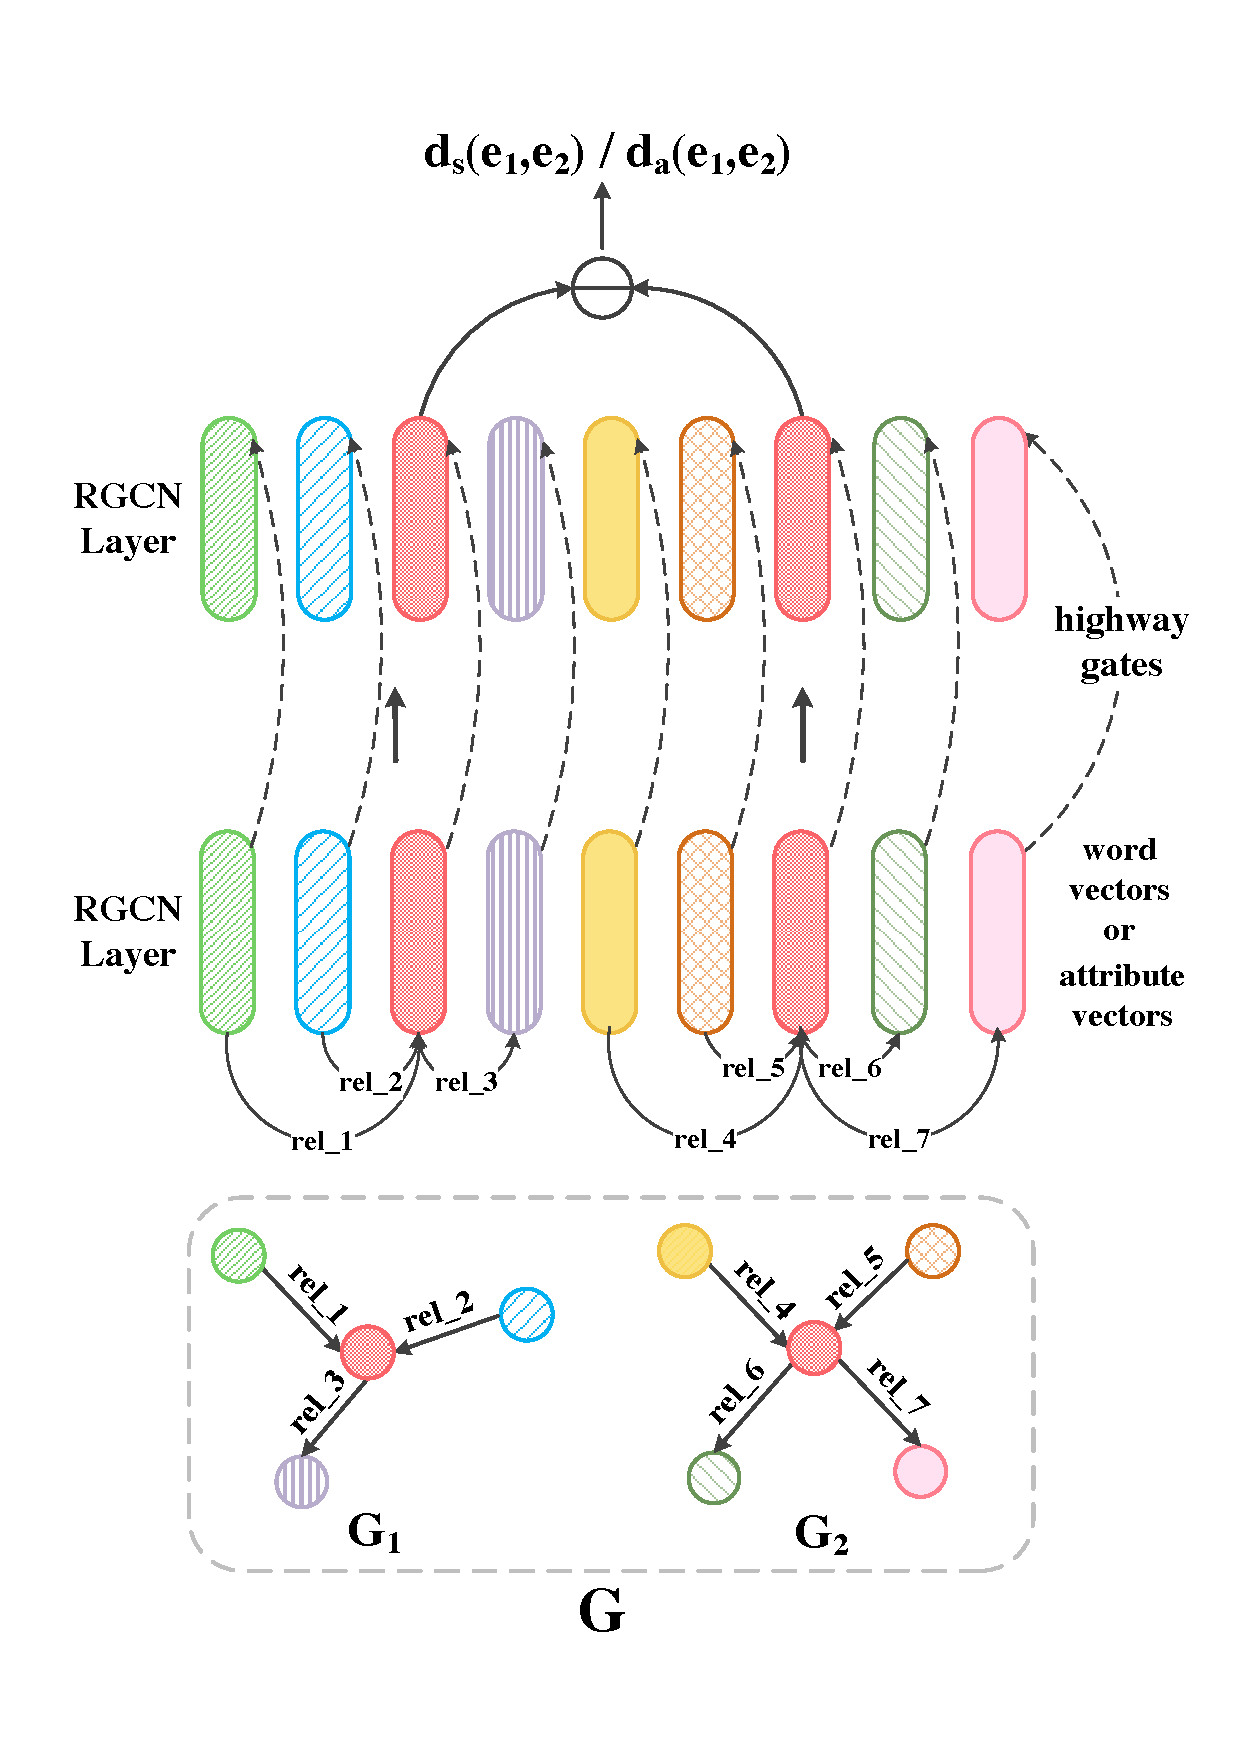
\includegraphics[width=0.8\linewidth]{figures/graph2.pdf}
			\caption{Overall architecture of our entity alignment model.}
			\label{all}
	\end{figure}
	
    \subsection{Base Model}
    Our approach is based on the recently proposed relational graph convolutional network (\RGCN)~\cite{Schlichtkrull2017Modeling}.
    \RGCN is an extension of Graph Convolutional Networks (\GCNs) that operate on local graph neighborhoods~\cite{Duvenaud2015Convolutional,Kipf2016Semi} to large-scale relational data.
    A \RGCN takes a set of adjacency matrices as input, and produces a new set of node features.
    Each input adjacency matrix describes the adjacency relationships among all nodes in the graph under each different relation.
    We choose to use \RGCN because it can model relational (directed and labeled) multi-graphs like \KGs.


 Our work improves \RGCNs in two ways. Firstly, we introduce highways to reduce the impact of noise (Section~\ref{section:hgcn}).
    Secondly, we use automatically learned semantic information such as entity names and attributes to improve the quality of the \KG
    embedding (Section~\ref{subsection:Node Representations}).


 %   Our work improves the featureless approach of \RGCN with pre-defined node feature vectors.
%    We believe that in addition to the internal structures, the semantic information of entity names and the attribute information of entities can help \RGCN better embed \KGs.
%    Therefore, we incorporate the aforementioned information into the node features as part of the model inputs.


	
	
	\subsection{R-GCN-based Entity Alignment}
	\label{section:rgcn}	

	The input to our \RGCN model are two parts. The first part is the node feature matrix $X^{(0)} \in \mathbb{R}^{N \times d^{(0)}}$ of $G$, where $N$ is the number of nodes and $d^{(0)}$ is the dimension of the input representations. We utilize predefined node features described in Section~\ref{subsection:Node Representations} to construct $X$ instead of using a featureless approach in \RGCNs~\cite{Schlichtkrull2017Modeling}.
	The second part is the list of adjacency matrices $A=\{A_1,A_2,...,A_R |A_i \in \mathbb{R}^{N \times N} \}$, which describes the adjacency relationships among $N$ nodes under $R$ different relations. We extract $R_0$ original relations from knowledge graphs, then we add reverse relations in order to pass information from the opposite direction; and add the self loop to retain information of the node itself. These together compose $R=2R_0+1$ relations.
	In each layer $l$, the input is $X^{(l)} = \{x^{(l)}_1,x^{(l)}_2,...,x^{(l)}_{N} |x^{(l)}_{i} \in \mathbb{R}^{d^{(l)}}\}$. The forward propagation is formulated as:
	\begin{equation}
	x_i^{(l+1)}=\mathrm{ReLU} (\sum\limits_{r \in R}\sum\limits_{j \in N_i^r}\frac{1}{|N_i^r|}W_r^{(l)}x_j^{(l)})
	\end{equation}
	Different from general \GCNs, \RGCNs introduce relation-specific transformations which depend on the type and direction of an edge. And this kind of propagation model can better characterize highly multi-relational data characteristic of realistic \KGs. Here $W_r^{(l)} \in \mathbb{R}^{d^{(l+1)} \times d^{(l)}}$ is the weight matrix of relation $r$. $N_i^r$ is the set of neighbor indices of node $i$ under relation $r$, according to normalized adjacency matrix $\hat A_r$. $\hat A_r$ is an approximate of spectral convolutions on $A^r$, introduced by ~\cite{Kipf2016Semi}:
	\begin{equation}
	\hat A_r=\hat D_r^{- \frac{1}{2}}(A_r+I)\hat D_r^{- \frac{1}{2}}
	\end{equation}
	where $(\hat D_r)_{jj}=\sum_k(A_r+I)_{jk}$.
	
	We get the new embedding matrix $X^{(l+1)} \in \mathbb{R}^{N \times d^{(l+1)}}$ by stacking the output $x_i^{(l+1)}$ together.
	
	As there are generally thousands of relation types in knowledge graphs, there will be a large amount of parameters to train and the model is likely to overfit. Hence we employ the basis decomposition, which is introduced in ~\cite{Schlichtkrull2017Modeling}, to regularize the weights:
	\begin{equation}
	W_r^{(l)}=\sum\limits_{b=1}^B a_{rb}^{(l)}V_b^{(l)}
	\end{equation}
	where $V_b^{(l)} \in \mathbb{R}^{d^{(l+1)} \times d^{(l)}}$ and $a_{rb}^{(l)}$ is the coefficient of matrix $V_b^{(l)}$ for relation $r$.
	

	\subsection{Node Representations}
	\label{subsection:Node Representations}
	There are two methods to initialize the node feature vectors.
	One way is to use the semantics of entity names, and the other is to use entities' attribute information. The specific initialization methods are as follows.
	
	\cparagraph{Semantic initialization}
	\label{wordvector}
	We believe that the names of entities and their counterparts in multiple \KGs should be semantically similar. Therefore we leverage the pre-trained word embeddings to introduce the semantic information about the names of entities.
	For Chinese datasets, we use word2vec software of Tomas Mikolov and his colleagues\footnote{https://code.google.com/archive/p/word2vec} to generate word embeddings. In our experiments, the window size is 5 and threshold for downsampling the frequent words is 20. Sentences in Baidu baike are used as training data and 4,200,006 100-dimensional word vectors are generated.
	
	\cparagraph{Attribute initialization}
	For attribute values, we distinguish four kinds of abstract range types, i.e., Integer, Double, Date and String (as default).
	In this paper, we only consider the first three types, i.e., Integer, Double and Date.
	We overlook String type values by reason of their complexity and heterogeneity in different \KGs.
	
	We construct normalized attribute vector for each entity.
	Specifically, the dimension of attribute vector is equal to the number of distinct attributes of which the value types belong to Integer, Double and Date in the \KG.
	The elements in an entity’s attribute vector equal to the normalized values of the corresponding attributes.
	If an entity does not have an attribute, the element corresponding to this attribute in the vector is then set to 0.
	
	Since it is the first attempt, we only consider the numerical part of a value, regardless of the unit, that is, we do not insist on normalizing \emph{1.80m} and \emph{180cm}.
	We leave this for future work.


	\subsubsection{Highway R-GCNs}
	\label{section:hgcn}
	While stacking RGCN layers makes our model capable of learning more neighborhood information from several relational steps, it may as well bring noise from the exponentially increasing neighbors. To reduce the effect of noise and ensure effective spread of more informative and discriminative neighborhood information, we add layer-wise gates similar to highway networks~\cite{Srivastava2015Highway} to our RGCN entity alignment model. ~\cite{Rahimi2018Semi} have successfully introduced highway gates to \GCNs~\cite{Kipf2016Semi} to solve the user geolocation problem. We introduce layer-wise highway gates to our RGCN model to finally get Highway RGCN (HRGCN) model and the output of a HRGCN layer is computed as:
	\begin{equation}
	\begin{split}
	&T(x^{(l)})=\sigma(W_T^{(l)}x^{(l)}+b_T^{(l)}) \\
	&x^{(l+1)}=x^{(l+1)} \cdot T(x^{(l)})+x^{(l)} \cdot (1-T(x^{(l)}))
	\end{split}
	\end{equation}
	where $\sigma$ indicates the sigmoid activation function, $\cdot$ is element-wise multiplication, $W_T^{(l)} \in \mathbb{R}^{d^{(l+1)} \times d^{(l)}}$ and $b_T^{(l)} \in \mathbb{R}^{d^{(l)} \times 1}$ are the weight matrix and bias vector of transform gate $T(x^{(l)})$.
	
	\subsection{Alignment Prediction}
	After HRGCN layers, we get the hidden representations $\bar{X}$ of all nodes in both \KGs. We measure the similarity between $e_1$ in $G_1$ and $e_2$ in $G_2$ by the distance between their hidden representations:
	\begin{equation}
	\label{d}
	d(e_1,e_2)=|\bar{x}_{e_1}-\bar{x}_{e_2}|
	\end{equation}
	, where $|\cdot|$ indicates the $l_1$ norm. The distance for equivalent entities is expected to be smaller than non-equivalent ones. In our experiments, for a entity $e_1$ in $G_1$, we computes the distances between $e_1$ and all the entities in $G_2$. The alignment process can also be reversed, i.e. from $G_2$ to $G_1$. Since, we report the results of both directions of entity alignment in our experiments.
	
	A set of pre-aligned entity pairs $\mathbb{L}$ and the set of negative pairs $\mathbb{L'}$  constructed by corrupting $(p, q)$, i.e. replacing $p$ or $q$ with a randomly chosen entity in $G_1$ or $G_2$ are used for training. To maximize the distance between positive and negative instances, we use the margin-based loss function:
	\begin{equation}
	L=\sum\limits_{(p,q)\in \mathbb{L}}\sum\limits_{(p',q')\in \mathbb{L'}}\mathrm{max}\{0,d(p,q)-d(p',q')+\gamma\}
	\end{equation}
	$\gamma > 0$ is a margin hyper-parameter separating positive and negative entity alignments.
	
	\subsection{Combination of Semantic Embedding and Attribute Embedding}
	As we introduced in Section~\ref{subsection:Node Representations}, there are two methods to initialize the input node feature vectors.
	When we leverage the pre-trained word embeddings to initialize the node feature vectors, we call HRGCNs acting semantic embedding.
	And when the nodes are initialized by attribute vectors, we call HRGCNs performing attribute embedding.
	Following the same architecture in Figure~\ref{all}, we do semantic embedding and attribute embedding for $G$ respectively.
	
	We integrate semantic embedding and attribute embedding by defining a combined distance $D$ for aligning entities:
	\begin{equation}
		D(e_1,e_2)=\frac{1}{m}[\omega d_s(e_1,e_2)+(1-\omega)d_a(e_1,e_2)]
	\end{equation}
<<<<<<< HEAD
	, where $m$ is the dimension of the new node features produced by HRGCNs.
	In our experiments, we set the output dimensions of two models (one for semantic embedding and the other one for attribute embedding) to be the same.
=======
	where $m$ is the dimension of the new node features produced by HRGCNs.
	In our experiments, we set the output dimensions of two models (one for semantic embedding and the other one for attribute embedding) to be the same.
>>>>>>> origin/master
	$\omega$ is a hyper-parameter. $d_s$ and $d_a$ are the distance computed by Eq.~\ref{d} according to semantic embedding and attribute embedding, respectively.
	
